\documentclass[11pt]{article}
\usepackage{cite}
\usepackage{graphicx}
\usepackage{hyperref}
\usepackage{amsfonts}
\usepackage{listings}

\begin{document}

\title{Odefying Kirkham}
\author{Simon Johanning}
\date{\today}
\maketitle

\tableofcontents

\section{Introduction} \label{sec:Intro}
\subsection{Background}
This course work has been written in the context of the course "Modellierung biologischer und molekularer Systeme" (WS 2015/16) at the University of Leipzig.

It is based on a presentation of the paper \textit{Early gene regulation of osteogenesis in embronic stem cells} by \textit{G.R. Kirkham et. al.} (see \cite{Kirkham}) in the context of aforementioned course.

It will lay out the basic ideas of the paper (\ref{ssec:Kirkham}), give an overview of the mathematical ideas the methodology is based upon (\ref{sec:Theory}), and will discuss results from the investigation of the boolean networks (\ref{sec:Results}). It will close with a discussion of the paper and the derived results (\ref{sec:Discussion}).

Since the course associated with this course work is about (mathematical) modeling, and the mathematical techniques used in the paper were merely sketched, this report will focus mostly on the mathematical ideas and modeling aspects employed in the paper, as well as the challenges in reproducing the results, and will only treat the biological context of \cite{Kirkham} on the side.
\subsection{Kirkham paper} \label{ssec:Kirkham}
\subsubsection{Motivation}
Motivated by the knowledge gap of networks regulating the differentiation of mouse embryonic stem cells into bone cells, the authors of \cite{Kirkham}, are interested in understanding the regulatory mechanisms of osteogenesis.
Since mathematical models of gene regulatory networks (GRNs) have proven to characterize GRNs well, as well as making novel predictions, especially in the case of incomplete data, the authors investigate mathematical models suited for this application.

Since boolean models (BMs) capture the qualitative dynamics of biological systems in a number of studies, the authors chose to start out modeling the GRN under investigation with boolean models.
In order to capture the quantitative dynamics of the system under investigation, they then transform these BMs into their continuous homologue functions in order to describe the system as a set of ordinary differential equations (ODE), a process call "odefication", using the \href{http://www.helmholtz-muenchen.de/icb/software/odefy/index.html}{Odefy} toolbox.

This process is chosen, since the description of a system through ODEs captures the dynamics of a system very well, and helps the authors to identify a (unique) GRN characterizing the influence of the transcription and growth factors under consideration.

\subsubsection{Structure}
As noted above, \cite{Kirkham} investigates GRNs relevant to osteogenesis in embryonic stem (ES) cells. Based on existing research on osteogenetic differentiation of mouse ES cells, they derive a set of three genes and two growth factors (GFs) to be of particular interest for this GRN, and aim to identify the relationship between them. 
These are the genes Runx2, Dlx5, Msx2 and the GFs TGF$\beta$1 and BMP2.

Consequently the authors test different GRNs involving these genes and GFs, narrowing down the possible candidates. 

Starting from modeling the GRNs as Boolean Models, they transform these into differential equations ("odefication") fitted to measured data in order to test predictions about the GRNs behaviour under over- and underexpression of the GFs. 

Their experimental data comprises a set of measurements of the TFs of interest (Dlx5, Msx2, Runx2) at 5 fixed time points, exposed to the GFs BMP2, TGF$\beta$1 and a combination of these.
The expression levels of the TFs were used to reduce the number of candidate GRNs through comparing the expression profiles to the stable states of the GRNs.

The remaining GRNs (i.e. the ones matching the experimental expression profiles), were then transformed into continuous ODEs, and their over- and underexpression behaviour was compared to experimental results, ruling out all but one network.

The paper closes with a discussion and the description of the experimental setup.

\section{Theory} \label{sec:Theory}
\subsection{Boolean Models}
As mentioned in the \hyperref[sec:Intro]{Introduction}, \cite{Kirkham} starts out with boolean models of the
species in the GRN. Boolean models (BMs) express qualitative biological knowledge, meaning that a species is either active or inactive (binary state). Represented as a graph (see \hyperref[regulatory_network]{figure 1}), the species are seen as nodes, whereas the interactions between the species are modeled as edges (which can be either activating, inhibatory or no influence).
Despite their coarseness, BMs can reproduce the qualitative behaviour of biological systems.
Due to their discrete nature however, they are not suited for quantitative models. Thus they can neither explain nor predict quantitative experiments, which is increasingly important in systems biology. For these applications,
the transformation to systems of ordinary differential equations (ODEs) has shown to be fruitful.

\subsubsection{Formal description}
Formally boolean models for N species $X_{1}, X_{2},..., X_{N}$, represented by variables $x_{i} \in \{0, 1\}$, are
defined by a set of species $R_{i} := \{X_{i_{1}}, X_{i_{2}},..., X_{i_{N_{i}}}\} \subset
\{X_{1},...,X_{N}\}$ influencing $X_{i}$, as well as an update function $B_{i}: \{0, 1\}^{N_{i}} \rightarrow \{0, 1\}$ for every combination of ($x_{i_{1}},..., x_{i_{2}}, x_{i_{N_{i}}}) \in \{0, 1\}^{N_{i}}$.

Mapped on the (hyper-) unit cube, the nodes ($\xi_{i_{1}},\xi_{i_{2}},..., \xi_{i_{N_{i}}}) \in \{0, 1\}^{N_{i}}$ corresponding to the domain of $B_{i}$, can logically be interpreted as $( \bigwedge_{ij| \xi_{ij = 1}} x_{ij} ) \wedge ( \bigwedge_{ij| \xi_{ij = 0}} \neg x_{ij} )$, meaning that $B_{i}$ will be true for the nodes of the cube where
the coordinate equals the boolean value of influence of the activation function.
With the sum-of-product representation, $B_{i}$ can now be viewed as: $B_{i} (x_{i_{1}}, x_{i_{2}},..., x_{i_{N_{i}}} ) = \bigvee_{(\xi_{i_{1}}, \xi_{i_{2}},..., \xi_{i_{N_{i}}}) | B_{i} ( \xi_{i_{1}}, \xi_{i_{2}},..., \xi_{i_{N_{i}}}) = 1} $ [ $( \bigwedge_{ij | \xi_{ij = 1}} x_{ij}) \wedge ( \bigwedge _{ij | \xi_{ij = 0}}  \neg x_{ij} ) $].

Thus each product can be represented  as a hyperedge between the start nodes $ S \subset \{X_{i_{1}}, X_{i_{2}},..., X_{i_{N_{i}}}\}$ and the end node $X_{i}$, with each pair $(s, X_{i}), s \in S$ carrying a sign on whether it is noted as a factor $x_{ij}$ or $\neg x_{ij}$ in the BM.

\subsection{General approach to make discrete models continuous} \label{ssec:prop}
In order to derive continuous models from the BMs, continuous homologues of $B_{i}$ have to be found. For this, the discrete variables $x_{i}$ are replaced by continous variables $\overline{x_{i}} \in [0, 1]$ , yielding the \textit{continuous homologue} functions $\overline{B_{i}} : [0, 1]^{N_{i}} \rightarrow [0, 1]$ on the unit interval.

Using the continous homologues of the BMs, the behavior of the species can be described through the differential equation

 $\dot{\overline{x_{i}}} = \frac{1}{\tau_{i}} (\overline{B}_{i} (\overline{x}_{i_{1}}, \overline{x}_{i_{2}},..., \overline{x}_{i_{N_{i}}}) - \overline{x}_{i})$,
 
 where the production of $\overline{x}_{i}$ is given by $\overline{B}_{i}$, and $\tau_{i} := \frac{1}{\gamma_{i}}$ stands for the life-time of species $X_{i}$, with $\gamma_{i}$ as the decay rate of $X_{i}$.

For the (in respect to the BM) homologuous continuous functions $\overline{B}_{i}$, three properties need to hold (as noted in \cite{Wittmann}):
\begin{itemize}
	\item \textbf{Accuracy}: $\overline{B_{i}}$ and $B_{i}$ need to agree on the vertices of the unit cube ($\{0,1\}^{N_{i}})$ \footnote{$\overline{B_{i}}$ are then called \textit{perfect} continuous homologues, exhibiting similar steady-state behavior}
	\item \textbf{Good analytical properties} such as smoothness, so a mathematical analysis as a system of ODEs can be performed
	\item \textbf{Minimality and uniqueness}: $\overline{B}_{i}$ should be the unique minimal solutions in their interpolation class
\end{itemize}

\subsubsection{HillCube}
In order to achieve the desired properties sketched above, normalized \textit{HillCubes} are constructed. HillCubes employ \textit{Hill functions} on the edges of the unit cube described above for the functional behavior of the interpolations.
As a first step to arrive at (normalized) HillCubes, \textit{BooleCubes} are constructed. These are functions that interpolate $B_{i}$ linearly through the use of multivariate polynomial interpolation. In order to get a unique solution,
the function with the minimal degree (of the polynomial) is chosen. This function satisfies the properties set out in \ref{ssec:prop}.

The functions $\overline{B}_{i}^{I} (\overline{x}_{i_{1}}, \overline{x}_{i_{2}},..., \overline{x}_{i_{N_{i}}} )$ define a system of ODEs that describes the temporal development of $\overline{x}_{i}$ through the equations 

$\dot{\overline{x}_{i}} = \frac{1}{\tau_{i}} (\overline{B}_{i}^{I} (\overline{x}_{i_{1}}, \overline{x}_{i_{2}},..., \overline{x}_{i_{N_{i}}}) - \overline{x}_{i} )$.

These \textit{BoolCube} functions are affine multilinear \footnote{$1 \leq j \leq N_{i} , \overline{x}_{ik}, k \neq j$ fixed: $ \exists a, b \in \mathbb{R} : \overline{B_{i}}^{I} (\overline{x}_{i_{1}}, \overline{x}_{i_{2}},..., \overline{x}_{i_{N_{i}}} ) = a + b \overline{x}_{ij}$}.
However, molecular interactions exhibit switch-like behavior rather than affine multilinear behavior. In order to model this, (sigmoid shape) \textit{Hill functions} $(f(\overline{x}) = \frac{\overline{x}^{n}}{ \overline{x}^{n} + k^{n}} )$ are used.

These functions are parameterized by the \textit{Hill coefficient} (n), that determines the slope of the curve and measures the cooperativity of the interaction, and the threshold where a species is considered as 'on' in the BM (k), thus where the value of activation is half maximal. Mathematically, the HillCube functions $\overline{B_{i}^{H}}$ are described through 

$\overline{B_{i}^{H}} (\overline{x}_{i_{1}}, \overline{x}_{i_{2}},..., \overline{x}_{i_{N_{i}}} ) := \overline{B}_{i}^{I} (f_{i_{1}}(\overline{x}_{i_{1}}), f_{i_{2}} (\overline{x}_{i_{2}}),..., f_{i_{n}} (\overline{x}_{i_{N_{i}}}) )$.

Since the Hill functions approach 1 only asymptotically, HillCubes are not perfect homologues of $B_{i}$, and not all desired properties sketched in \ref{ssec:prop} are fulfillled. Thus, in the odefy-approach, the Hill functions are subsequently normalized on the unit interval. HillCubes $\overline{B}_{i}^{H_{n}}$ are defined by $\overline{B}_{i}^{H_{n}} (\overline{x}_{i_{1}}, \overline{x}_{i_{2}}, ..., \overline{x}_{i_{N_{i}}}) := \overline{B}_{i}^{I} ( \frac{f_{i_{1}}(\overline{x}_{i_1})}{f_{i_{1}} (1)}, \frac{f_{i_{2}}(\overline{x}_{i_2})}{f_{i_{2}} (1)}, ..., \frac{f_{i_{N_{i}}}(\overline{x}_{i_{N_{i}}})}{f_{i_{N_{i}}} (1)})$.

The value of the Hill function $f_{i_{j}}$ on the value 1 thus normalizes the HillCubes on the unit interval. Normalized HillCubes yield a perfect continuous homologue of the Boolean functions $B_{i}$. Thus, a steady-state of the BM will
also be a steady-state of the continuous system \footnote{This exemplifies the importance of normalization, since steady-states of the BM are not (necessarily) steady-states of the non-normalized HillCubes.}, as shown in \cite{Wittmann}. However, the authors note that this method does not accurately transform the Boolean update rule into a continuous activation function. 

This is due to a systematic difference between the Boolean logic and the analytic form of the activation function (see \cite{Wittmann}). For the HillCube models, the imperfect agreement is caused by the asymptotic behavior of the Hill
functions, and thus can be made arbitrarily small (through the appropriate choice of parameters), justifying the described approach.

\subsection{Odefy}
\href{http://www.helmholtz-muenchen.de/icb/software/odefy/index.html}{Odefy}, a MATLAB and GNU Octave compatible toolbox for the "odefication" (transformation into continous ODEs) of boolean models, has been developed by the \href{http://www.helmholtz-muenchen.de/icb/index.html}{Institute for Computational Biology of the Helmholtz-
Zentrum M{\"u}nchen}.

ODEs allow for a more detailled and quantitative characterization of GRNs. Qualitative (biological) knowledge is represented as BMs, which are transformed into continuous model, that are fitted with quantitative data (see \hyperref[odefy_workflow]{figure 2}).

Odefy uses the HillCube modeling technique. With $\overline{B}_{i}$ as the HillCube model of $\overline{x}_{i}$, the following differential equation is reached: $\dot{\overline{x}}_{i} = \frac{1}{\tau_{i}} (\overline{B}_{i} (\overline{x}_{i_{1}}, \overline{x}_{i_{2}},..., \overline{x}_{i_{N_{i}}} ) - \overline{x}_{i} )$, where $\tau_{i}$ stands for the lifespan of species $X_{i}$ (as described in \ref{ssec:prop}).

\begin{figure}[hb]
  \centering
  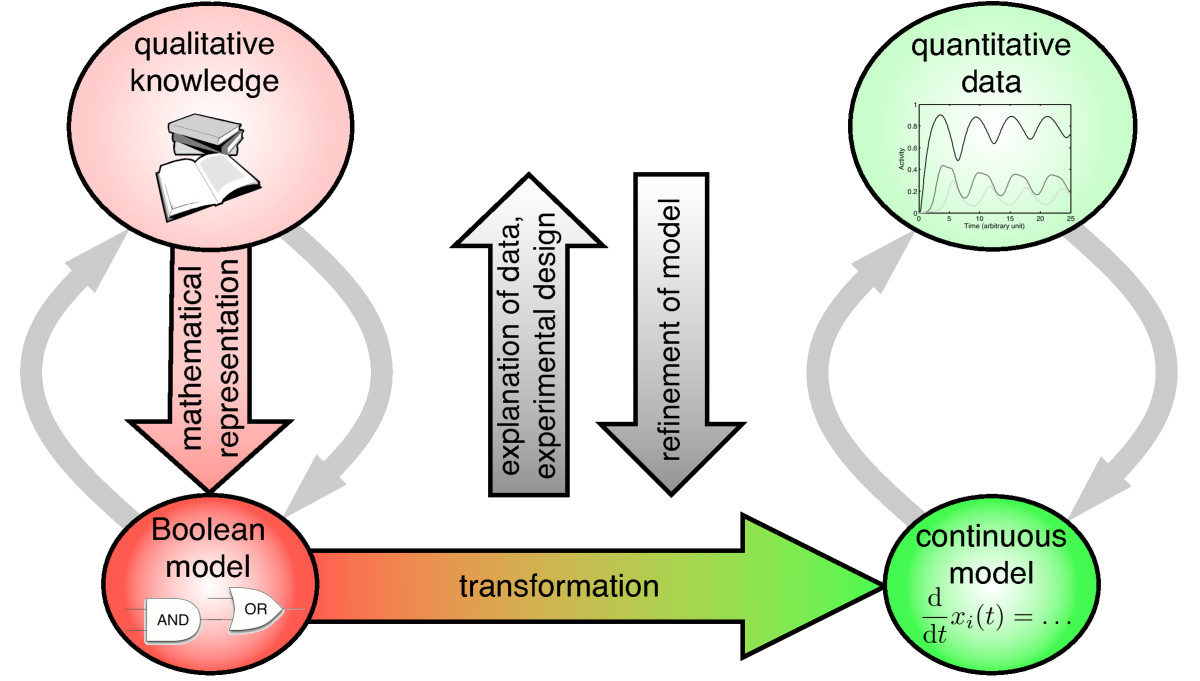
\includegraphics[width=0.65\textwidth]{odefy.jpg}
  \caption{\label{odefy_workflow} Sketch of the odefy workflow.}
\end{figure}

\section{Results} \label{sec:Results}
The simulations were realized with the Odefy 1.19 toolbox in \href{https://www.gnu.org/software/octave/}{GNU Octave}
4.0.0. To follow the workflow of the study, first the candidate networks depicted in \hyperref[regulatory_network]{figure 1} were created. Subsequently the continuous models were simulated.

\subsection{Creation of the BM} \label{ssec:creation}
The candidate BM, as derived from the literature (see also \hyperref[regulatory_network]{figure 1}), use the GFs
BMP2 and TGF$\beta$1, as well as the genes Dlx5, Msx2 and Runx2.
Since the authors assumed that the influence of TGF$\beta$1 to Msx2, BMP2 to Msx2 and Dlx5, as well as the influence of Dlx5 on Runx2 was activatory, the following substrings are fixed in the model description (odefy-syntax):
'Msx2 = TGF$\beta1$ $||$ MBP2', 'Dlx5 = BMP2', 'Runx2 = Dlx5' \footnote{Meaning that for LHS = RHS the LHS is considered 'on' iff the RHS is (and 'off' otherwise).}.
To model the unclear relations under investigation, 5 variables are used, where the value -1 represents an inhibatory relation, 0 no influence of the first factor onto the second and 1 as activatory influence. The variables used are as follows:

\begin{tabular}{c c c}
\textbf{variable} & \textbf{biological meaning} & \textbf{value} \\
\hline
Msx2Dlx5 & Influence of Msx2 on Dlx5 & (index / $3^{0}$) \% 3 - 1 \\
Dlx5Msx2 &  Influence of Dlx5 on Msx2 & (index / $3^{1}$) \% 3 - 1 \\ 
Msx2Runx2 &  Influence of Msx2 on Runx2 & (index / $3^{2}$) \% 3 - 1 \\ 
TGFb1Runx2 &  Influence of TFG$\beta$1 on Runx2 & (index / $3^{3}$) \% 3 - 1 \\ 
Runx2Dlx5 &  Influence of Runx2 on Dlx5 & (index / $3^{4}$) \% 3 - 1 \\
\end{tabular}

\subsubsection{Model creation}
The BMs specified above are 'odified' through the \textit{ExpressionsToOdefy} command of the odefy toolbox. This command requires an expression describing the boolean network. For every candidate configuration of the GRN (see \hyperref[regulatory_network]{figure 1}), the interactions of the species are modeled. For all three genes, the relevant
interactions are either added as activatory (x), left out or added as inhibitory ( $\tilde{} x$).

For this project, default parameters were chosen \footnote{n=3, k=0.5, $\tau$=1, according to \cite{Krumsiek}} , since no parameters were reported in \cite{Kirkham}, and it is to be expected that default parameters were used in the publication. The following source code exemplifies how the expressions are constructed:

\begin{lstlisting}
models = [0:242]
for index = [0 : 242]

# behavior of Msx2
Msx2String = "Msx2 = TGFb1 || BMP2";
if(rem(floor(index / 3), 3) - 1 == -1)
	Msx2String = [Msx2String, " || ~Dlx5"];
elseif(rem(floor(index / 3), 3) - 1 == 1)
	Msx2String = [Max2String, " || Dlx5"];
endif

# behavior of Dlx5
Dlx5String = "Dlx5 = BMP2"
#	influence of Msx2
if(rem(floor(index), 3) - 1 == -1)
	Dlx5String = [Dlx5String, " || ~Msx2"]
elseif(rem(floor(index), 3) - 1 == 1)
	Dlx5String = [Dlx5String, " || Msx2"]
endif
#	influence of Runx2
if(rem(floor(index / 81), 3) - 1 == -1)
	Dlx5String = [Dlx5String, " || ~Runx2"]
elseif(rem(floor(index / 81), 3) - 1 == 1)
	Dlx5String = [Dlx5String, " || Runx2"]
endif

# behavior of Runx2
Runx2String = "Runx2 = Dlx5"
#	influence of Msx2
if(rem(floor(index / 9), 3) - 1 == -1)
	Runx2String = [Runx2String " || ~Msx2"]
elseif(rem(floor(index / 9), 3) - 1 == 1)
	Runx2String = [Runx2String " || Msx2"]
endif
#	influence of TGFb1
if(rem(floor(index / 27), 3) - 1 == -1)
	Runx2String = [Runx2String " || ~TGFb1"]
elseif(rem(floor(index / 27), 3) - 1 == 1)
	Runx2String = [Runx2String " || TGFb1"]
endif

# construct model string
	expressionString = ["BMP2 = <>,", " TGFb1 = <>, ",Msx2String, ", ", Dlx5Strin
# construct BM for odefy
expression = {"BMP2 = <>", " TGFb1 = <>",Msx2String, Dlx5String, Runx2String};
model = ExpressionsToOdefy(expression);
models(index) = model
endfor
\end{lstlisting}

As mentioned in \cite{Krumsiek}, the boolean update functions are accessable as multidimensional arrays (hypercubes of edge length two). These are accessable through
\begin{lstlisting}
model.tables(x).inspecies
\end{lstlisting}

for a list of species that influence the species, and
\begin{lstlisting}
model.tables(x).truth
\end{lstlisting}

for the truth table for the expression the model was based upon. In the above code snippets, x stands for the index of the table struct to be accessed. Using \textit{ExpressionToOdefy}, the full BM is stored as an Odefy-internal representation with Octave.

\subsection{Simulation of continuous models} \label{ssec:simulationCM}
After the construction of the BM sketched above, simulations of the networks are performed using the \textit{OdefySimulation} ommand. This command takes a simstruct as parameter which has to be constructed from the models using the \textit{CreateSimstruct} command. The code thus is as follows:
\begin{lstlisting}
# construct struct for simulation
simstruct = CreateSimstruct(model);
simstruct.type = 'hillcubenorm';
# set presence of BMP2
simstruct = SetInitialValue(simstruct,'BMP2',1);
# set presence of TGFb1
simstruct = SetInitialValue(simstruct,'TGFb1',0);
# simulate
simres = OdefySimulation(simstruct);
plot(simres);
legend(model.species);
xlabel('time');
ylabel('expression')
\end{lstlisting}

The \textit{simstruct} is a data structure that holds the information required for the simulation, like initial states, simulation type and parameters.

In the example above, the initial values of the GFs are set arbitrarily to 'on' (BMP2) and 'off' (TGF$\beta$1) to exemplify the simulation run in the \textit{BMP2 only} environment. This is set purely for illustrative purposes, and all three
setups of the environment presented in \cite{Kirkham} are employed in the simulation. The \textit{type} attribute of the simstruct specifies that the normalized HillCube variant is employed.

The simulation is invoked by the \textit{OdefySimulation} function that takes the simstruct as parameter. Consequently, the expression of the species used is plotted.

\section{Discussion} \label{sec:Discussion}


\section{Representation of gene regulatory networks}
In \cite{Kirkham}, 243 possible GRN candidates are derived from the literature, namely the GRNs that differ in the mutual influence between Msx2 and Dlx5, the influence of TGF$\beta$1 and Msx2 on Runx2, and the influence of Runx2 on Dlx5
(see \hyperref[regulatory_network]{figure 1} for a graphical representation of the initial GRNs).
The GRNs are derived from literature, where two or more studies confirming the influence of one species upon another is understood as certain influence (i.e. no GRNs are generated that indicate no or contrary influence), one study reporting an influence is seen as unclear (dotted lines in \hyperref[regulatory_network]{fig. 1}, thus all three possible modalities are tested), and no reported finding is interpreted as no influence of one species unto another.

\begin{figure}[hb]
  \centering
  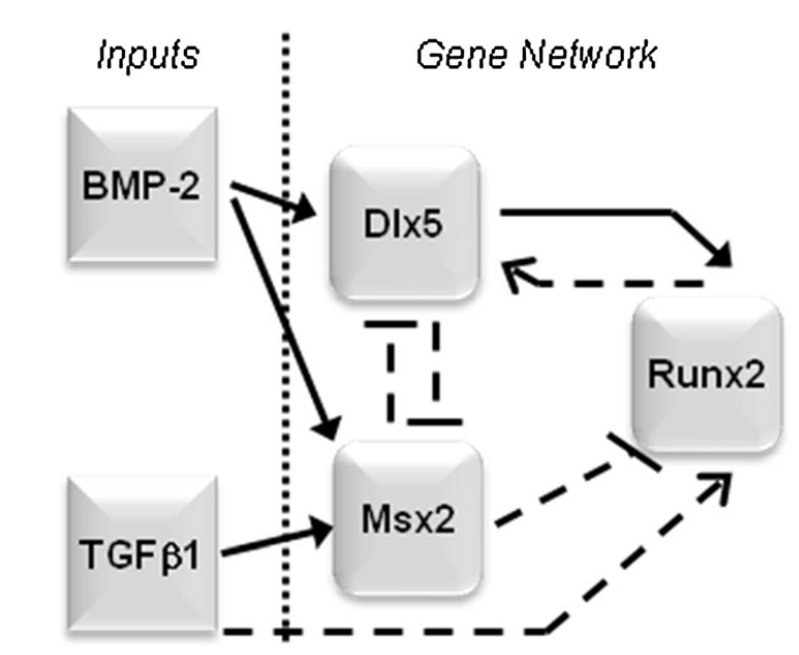
\includegraphics[width=0.8\textwidth]{regulatory_network.jpg}
  \caption{\label{regulatory_network} initial GRN as in \cite{Kirkham}. Dotted lines indicate an unclear influence of one species onto another.}
\end{figure}

\bibliography{references}{}
\bibliographystyle{plain}
\end{document}
